\documentclass{article} % latex file 
\usepackage[margin={1in}]{geometry}
\usepackage{amsmath} % For maths
\usepackage{amssymb} % For maths
\usepackage{graphicx} % For images
\usepackage{listings} % For Code boxes
\graphicspath{ {./images/} }

\title{CSU44012 Project 2: MineSweeper}
\author{Name: Alexander Sepelenco\\Student Number: 20335014}
\date{} % no date

\begin{document}
\maketitle
\tableofcontents

\section{Introduction}
I have completed mostly all tasks specified one implementation I would like to empahise later would be my solver which has a partial implementation, 
these tasks are: Phase 1, and Phase 2. Modelling the game of minesweeper, 
while developing I created a terminal game using this for debugging. Some source code for the terminal interactions exist,
but that can be ignored. I have also build the programme in threepenny gui. I have documented my source code by commenting
each function. Lib.hs contains the minesweeper logic while Main.hs contains the threepenny related code.

\subsection{Phase 1}
\subsubsection{MineSweeper implementation}
My Minesweeper implementation had these types and data constructors
\begin{itemize}
    \item type Width = Int
    \item type Height = Int
    \item type Row = [Square]
    \item type Board = [[Square]]
    \item type Location = (Int, Int)
    \item type Game = (Board, Location)
    \item data Square 
\end{itemize}
where Square has derived Show and Eq class for usability in other functions. The values of Square are: 
\begin{itemize}
    \item Empty
    \item Mine 
    \item Hidden
    \item Number Int
    \item Mark
\end{itemize}
The square here can be thought of as a tile. A tile in a minesweeper game can either by empty, have a mine, be hidden (for the player),
have some number which I represent with an Int, and a Mark (which is a flag) meaning a tile can be flagged. I use all these representations
so that I can create two board later. A board is the board the player sees, and another board which is where all the tiles are filled in
which I call the logicGame (lG) in my source code. In a typical game of minesweeper there are random locations of mines. I place mines
in an empty board if the same location exists I look for another random location (note, if we try to place more mines than the board allows
because of my "take" function and nub from Data.List I will loop indefinitely). This randomness requires IO actions which I will later use
liftIO operations on to work on the threepenny-gui. Selecting random tiles were based off the time. and time+1 for x and y respectively. 
\begin{itemize}
    \item Empty
    \item Mine 
    \item Hidden
    \item Number Int
    \item Mark
\end{itemize}

\subsection{Threepenny-gui}
Threepenny-gui had an official Github with multiple examples and Hoogle which documented the functions, it made making a simple 
user interactable web app doable. With Threpenny-gui I did not end up with going with the Functional part of threepenny, instead I worked with the
imperative part of threepenny. This means I created handlers for buttons such as on click for UI.buttons, and on mousedown for the canvas.
I used the canvas I drew lines on the grid using canvas related function provided in Threepenny-gui. I calculated the locations of the tiles
based of width and height of the board, and the game logic was used in the handlers. Using IORef's I was able to writeIORef (write) and readIORef (read)
and liftIO to match type of UI my uisetup my gui.

\section{Phase 2}
This was part was challenging. Creating a solver which "plays a move" button ended up being a difficult task. The task was to make a solver make an obvious
logical move guaranteed to not click a mine, and if that does not exist it will make a probabilistic guess. Unfortunately I did not end up creating a 
probabilistic computation by enumerating all possible mines on the empty tiles and finding the board with the highest variation and selecting that as a
board to click. Instead I went with making a guess. I can avoid using IO or random, I can make a random guess by just selecting the first hidden tile.
This is just as random as selecting any hidden tile. My logic solver uses the help of a player, the player will mark a spot they know is a mine, and the solver
will then calculate the surroundings that will not result in a mine, because it is pretty obvious it will reveal multiple a bunch of tiles, many times in 
the solver you can click solve again for it to make the obvious move that won't be a mine, this can speed up the playing of mine sweeper drastically.

\section{Reflection}
Generally speaking I found this project more challenging than the first. Nearly all parts had me in need of solving problems where as the previous
project most of the issues lied in the polygon drawing algorithm. When creating this project I had many hurdles particularly in the Threepenny-gui
part of the project. I initially started with created a grid of buttons rather than the canvas and mapping coordinates of the canvas to the tiles.
In Threepenny if I create a new body with a canvas the handlers stay they same but if I were to do that with buttons, the handlers are void, they 
become useless threepenny doesn't realise that these buttons are the same. So after making a huge shift from a button grid to a canvas I was able
to work more smoothly. I just needed to get practice with using IORef's to help with modifying my variables (my board games). 

\subsection{Design}
Coming from a very imperative mindset it was a bit harder to create useful functional solutions to the minesweeper solution. Instead I came from 
the angle of making functions which underutilized many of the features I could have used. Using lists for the minesweeper solution caused more 
of a headache. Partly at my fault for not making a new data type, traversing lists and make new boards after placing a single element is extremely inefficient
of time and memory. Since Haskell is pure it was harder to debug the classic way and so I was required to use the repl which proved to be more annoying
than C (my language of choice). But with the case of the library, despite functional programming it is definitely easier than something like C when 
it comes to graphics. But if I were to use a language with many resources and is used for the web primarily, javascript I think it could've been easier.
I don't think Threepenny-gui is a great way to develop simple web applications. Having pure functions definitely helped with correctness. Developing the
app resulted in less bugs than making an imperative programme. While developing once I matched type signatures I was almost guaranteed to get the expected
output which is what I like about Haskell. Threepenny-gui had multiple examples on their github which was nice when using the library. 
Testing was done through repl, I decided against using a testing library such as hproof, which I've used in projects before. 
Creating test cases takes a lot of time and I was more focused on getting it done as I have a tight schedule and start my internship on the 8th of 
January and have family and friend events planned before the date.

\section{Demo Video}
I have attached a video demo presentation of my programme. In the folder Documentation/ which will be in the zip I will attach.
\begin{figure}[h]
  \centering
  \begin{minipage}{0.3\textwidth}
    \centering
    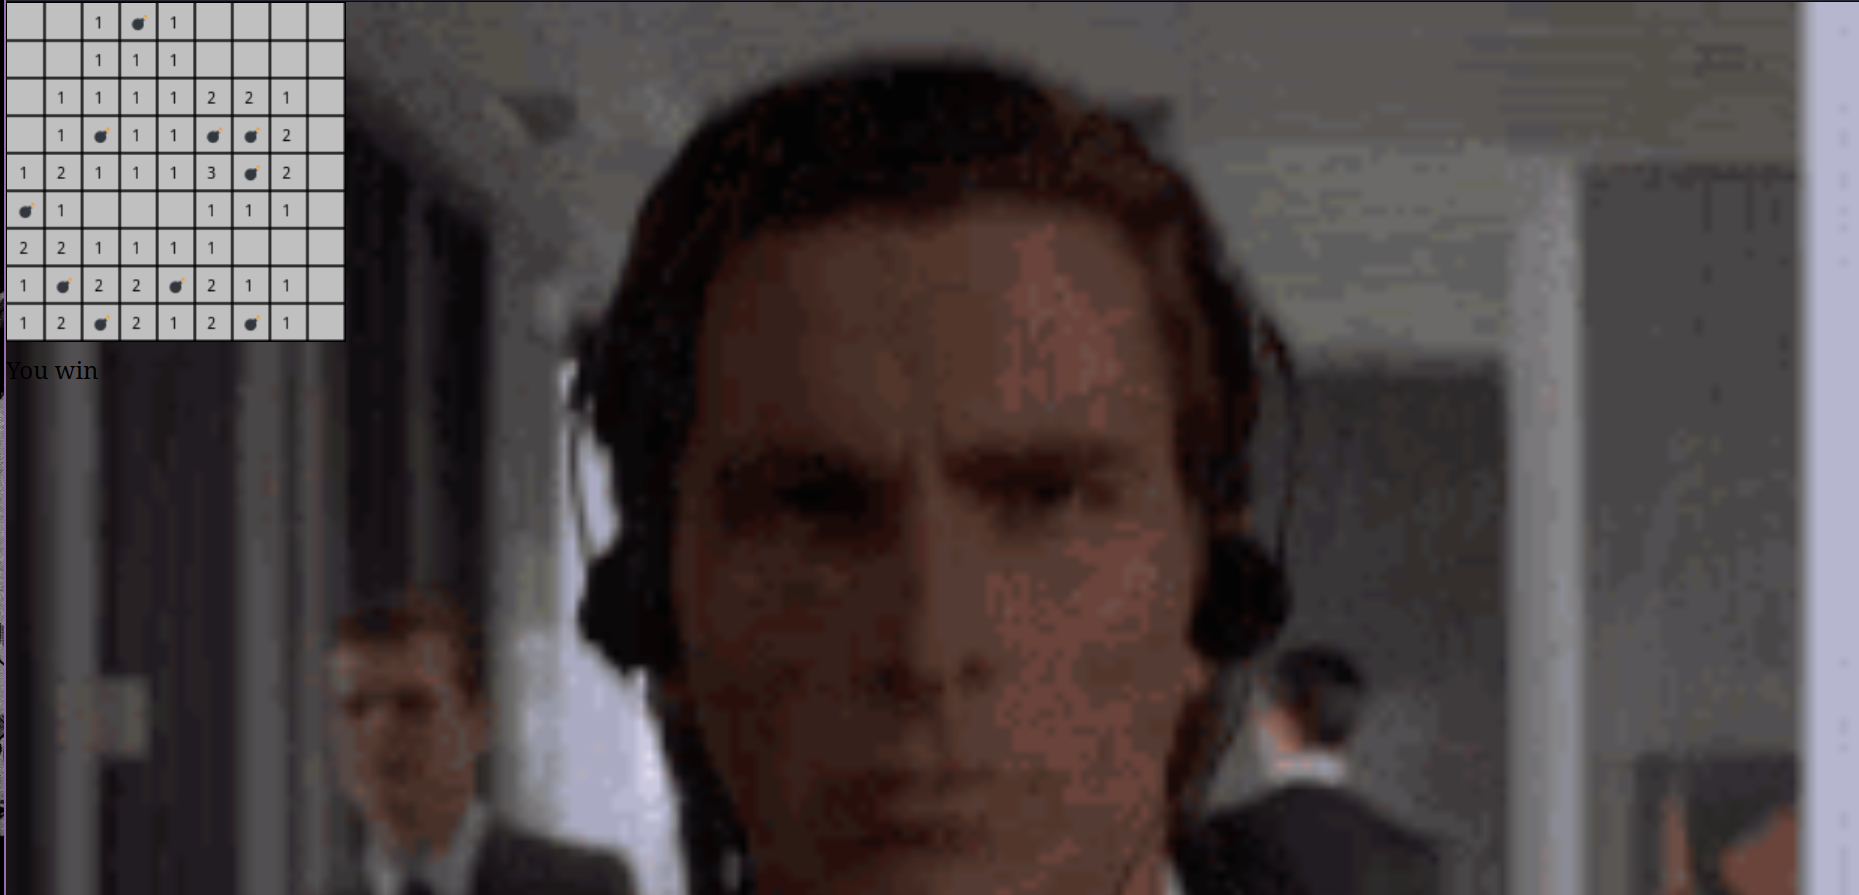
\includegraphics[width=1.0\linewidth]{youwin}
    \caption{You win Screen}
  \end{minipage}
  \begin{minipage}{0.3\textwidth}
    \centering
    
\includegraphics[width=1.0\linewidth]{gameover}
    \caption{Game Over Screen}
  \end{minipage}
  \begin{minipage}{0.3\textwidth}
    \centering
    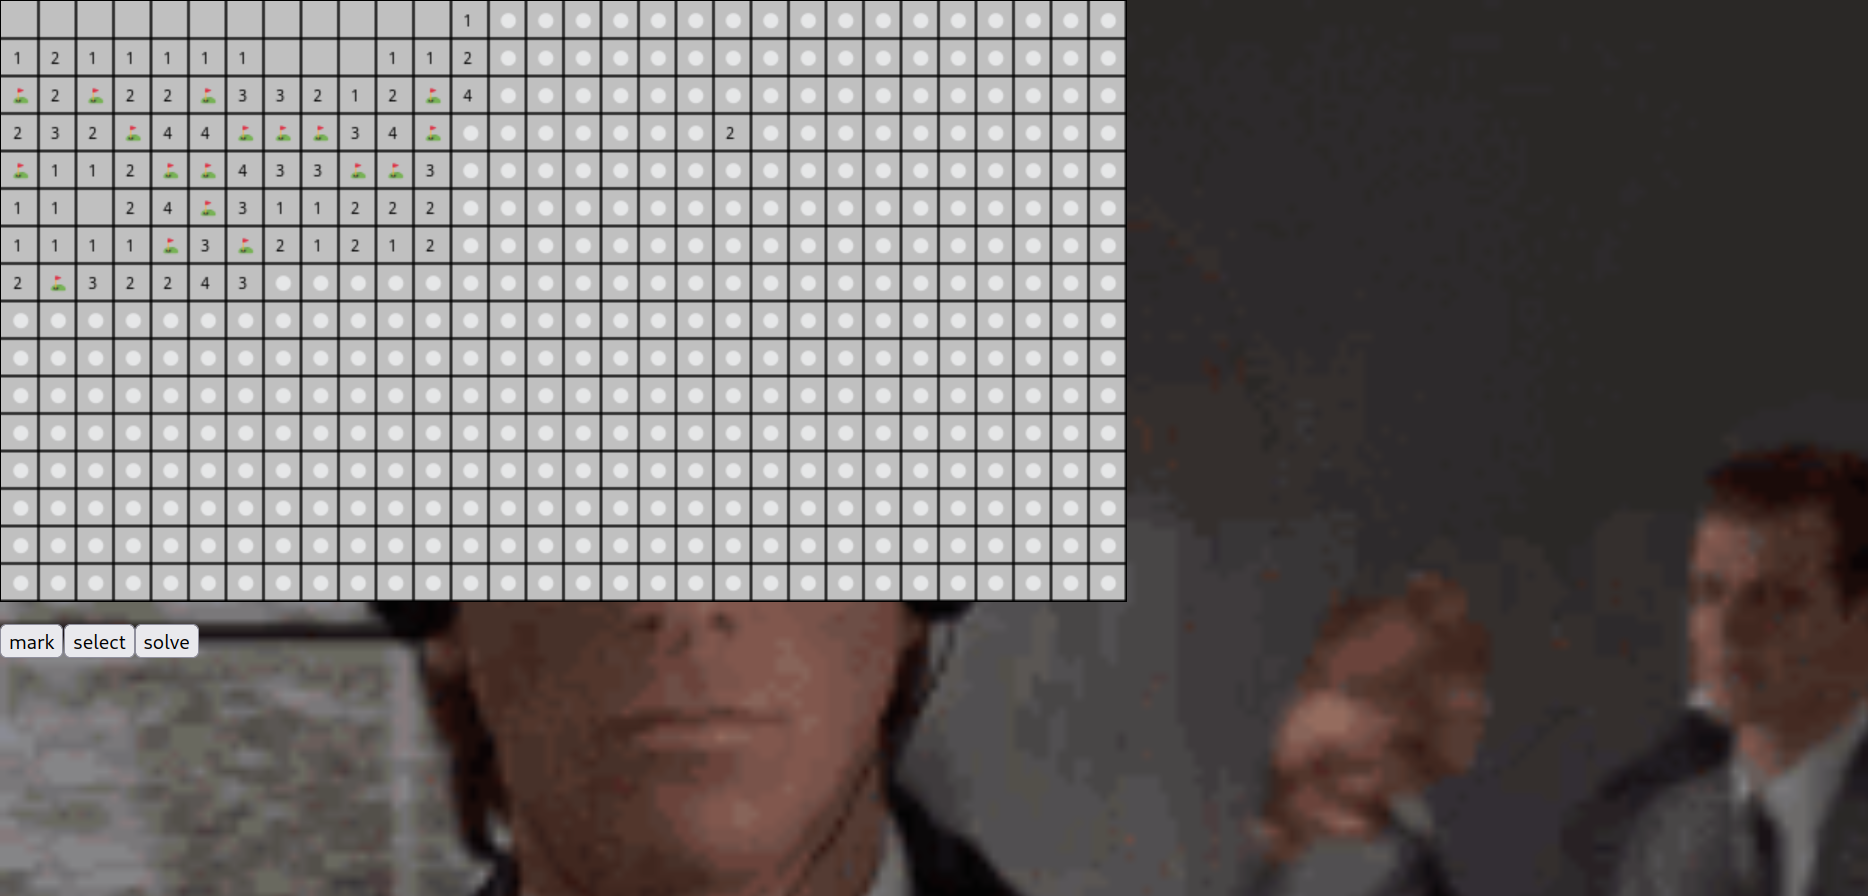
\includegraphics[width=1.0\linewidth]{expertboard}
      \caption{Expert Board}
  \end{minipage}
  \caption{Three Images Side by Side}
  \label{fig:three_images}
\end{figure}


\section{Bugs and Issues}
\begin{itemize}
    \item Clicking on the very edges of the canvas can cause the programme to consider it an invalid coordinate, this is unlikely to occur as it's 1 pixel or so
          wide, but with trying to fix the issue, I couldn't seem to get it working despite attempts at preventing an index out of the grid.
    \item The solver sometimes can reveal empty spots, if it does and doesn't reveal all hidden spots which is clear by seeing that an empty spot is beside a hidden
          tile, then you should press solve again.
    \item When using the solver as the last move, press solve once more when finished to mark to trigger the handler of checking the game condition was finished.
\end{itemize}

\end{document} 

